%! Author = schba
%! Date = 2023. 09. 16.

% Preamble
\documentclass[a4paper, 12pt]{article}

% Packages
\usepackage[magyar]{babel}
\usepackage{t1enc}
\usepackage[utf8]{inputenc}
\usepackage{lmodern}
\usepackage[pdftex]{graphicx}
\usepackage[lflt]{floatflt}
\usepackage{epstopdf}
\usepackage{amsmath,amssymb}
\usepackage{icomma}
\usepackage{array}
\newcolumntype{L}{>{$}l<{$}} % math-mode version of "l" column type
\usepackage[unicode,colorlinks]{hyperref}
%\usepackage{fullpage}
\usepackage{booktabs}
\usepackage{fancyhdr}
%\usepackage{subfigure}
\hypersetup{allcolors=black}
\hypersetup{pdfstartview=FitH}
\usepackage{float}
\usepackage{titling}
\usepackage{caption}
\usepackage{subcaption}
\usepackage{upgreek}
\usepackage{mhchem}
\usepackage{lstdoc}
\usepackage{amstex}

\title{\textbf{Hőmérsékleti Sugárzás Mérése}}
\author{Györgyfalvai Fanni ( \texttt{BKOGIJ)}, Schäffer Bálint ( \texttt{RHB36D)}
}
\date{2023.\ 09.\ 14.}

\frenchspacing
\widowpenalty=10000 \clubpenalty=10000
\setcounter{section}{-1}
\pagestyle{fancy}
\fancyhf{}
\fancyhead[L]{\nouppercase{Hőmérsékleti Sugárzás}}
\fancyhead[R]{\nouppercase{\leftmark}}
\fancyfoot[C]{\hfill\thepage\hfill}

% Document
\begin{document}
    \maketitle
    \tableofcontents
    \newpage

    \section{Elméleti Összefoglaló}\label{sec:elmeleti-osszefoglalo}
    \subsection{A hőmérsékleti sugárzás alapjai}\label{subsec:a-homersekleti-sugarzas-alapjai}
    Tapasztalati tény, hogy a testek, bennük atomi szinten lezajló folyamatok révén folyamatosan \textit{elektromágneses sugárzást} bocsátanak ki.
    Ezen elektromágneses sugárzás intenzitását elsősorban a test hőmérséklete határozza meg, csak úgy, mint a kibocsátott sugárzás spektrális eloszlását.
    Nem véletlen tehát, hogy ezt a jelenséget \textbf{hőmérsékleti sugárzásnak} nevezzük.

    Egy test által hőmérsékleti sugárzással kibocsátott energiát az \textit{emiszzióképességgel} ($\epsilon$) jellemezzük.
    Ez megadja, hogy az adott test $T$ hőmérsékleten egy $\lambda$ körüli $\Delta\lambda$ hullámhossztartományban egy $\Delta A$ nagyságú felületről $\Delta t$ idő alatt mennyi ($\Delta E$) energiát sugároz ki, azaz:
    \begin{equation}
        \varepsilon(\lambda, T)=\frac{\Delta E}{\Delta A\Delta t\Delta\lambda}.\label{eq:0eps}
    \end{equation}
    A teljes spektrumban kisugárzott (felületre és időre normált) energiát pedig ennek integrálásával kaphatjuk meg:
    \begin{equation}
        E(T)=\int_{0}^{\infty} \varepsilon(\lambda, T)~\mathrm{d}\lambda.\label{eq:0E}
    \end{equation}
    Hasonlóan definiálhatjuk egy elektromágneses hullám esetében az energia-áramsűrűséget, vagy ismertebb nevén\textit{intenzitást}:
    \begin{equation}
        I(\lambda)=\frac{\Delta E}{\Delta A\Delta t\Delta\lambda}.\label{eq:0I}
    \end{equation}
    A sugárzás teljes intenzitását pedig ezen infinitezimális intenzitások összegeként kapjuk:
    \begin{equation}
        I_0=\int_{0}^{\infty} I(\lambda)~\mathrm{d}\lambda.\label{eq:0I0}
    \end{equation}
    \begin{figure}[H]
        \centering
        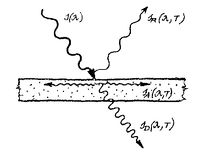
\includegraphics[width=5cm]{200px-Fenytores_homsug}
        \caption{Az elektromágneses sugárzás szétbomlása anyaggal való kölcsönhatás esetén \cite{leir}}
        \label{fig:0em}
    \end{figure}

    Ha a fogadó oldalt nézzük, egy testet érő elektromágneses sugárzással három dolog történhet: áteresztődik ($I_t(\lambda, T)$), elnyelődik ($I_a(\lambda, T)$), vagy visszaverődik ($I_r(\lambda, T)$), ahogy ezt~\aref{fig:0em}. ábrán is láthatjuk.
    Természetesen ez a három jelenség egyszerre lép fel a kölcsönhatások legnagyobb részében, így a végbemenetelüket valamilyen arányszámmal tudjuk jellemezni:
    \begin{align}
        &\xi(\lambda, T)=\frac{I_\xi(\lambda, T)}{I(\lambda)}; &\xi\in\{t, a, r\} \\
        &\xi(T)=\frac{\int_{0}^{\infty} I_\xi(\lambda, T)~\mathrm{d}\lambda}{\int_{0}^{\infty} I(\lambda)~\mathrm{d}\lambda}=\frac{I_\xi(T)}{I_0}.\label{eq:0intabs}
    \end{align}
    Ezeket rendre \textit{transzmisszió}-, \textit{abszorpció}- és \textit{reflexióképességnek} nevezzük.
    Mindet tudjuk definiálni integrált esetben is, ahogy \aref{eq:0intabs}. egyenletben látható.
    Az energiamegmaradásból következik, hogy a teljes intenzitás is megmarad, így:
    \begin{align}
        &t(\lambda, T)+a(\lambda, T)+r(\lambda, T)=1 \\
        &t(T)+a(T)+r(T)=1.
    \end{align}

    \subsection{Az abszolút fekete test}\label{subsec:az-abszolut-fekete-test}
    A testek sugárzásának vizsgálatához célszerű bevezetni egy absztrakciót (valójában ilyen test nem létezik), melyet \textbf{abszolút fekete testnek} hívunk.
    Ennek a legfontosabb tulajdonsága, hogy minden ráeső elektromágneses sugárzást elnyel, így felírható:
    \begin{equation}
        a(\lambda, T)=a(T)=1\equiv a_f.
    \end{equation}
    Fontos, hogy a fekete test által kisugárzott energia spektruma elméleti megfontolásokkal levezethető (\textit{Max Planck}, 1900 \cite{planck}):
    \begin{equation}
        \varepsilon_f(\lambda, T)=\frac{2hc^2}{\lambda^5}\frac{1}{e^{\frac{hc}{\lambda k_BT}}-1},
    \end{equation}
    ahol $h$ a Planck-állandó, $c$ a fénysebesség és $k_B$ a Boltzmann-állandó. Ez a \textbf{Planck-féle sugárzási törvény}.
    A megfelelő hullámhosszfüggés néhány hőmérsékleten \aref{fig:0blackrad}. ábrán látható. A maximumokra érvényes továbbá a \textbf{Wien-féle eltolódási törvény}, mely szerint:
    \begin{equation}
        \lambda_{\mathrm{max}}\cdot T=\mathrm{const}.
    \end{equation}
    \begin{figure}[H]
        \centering
        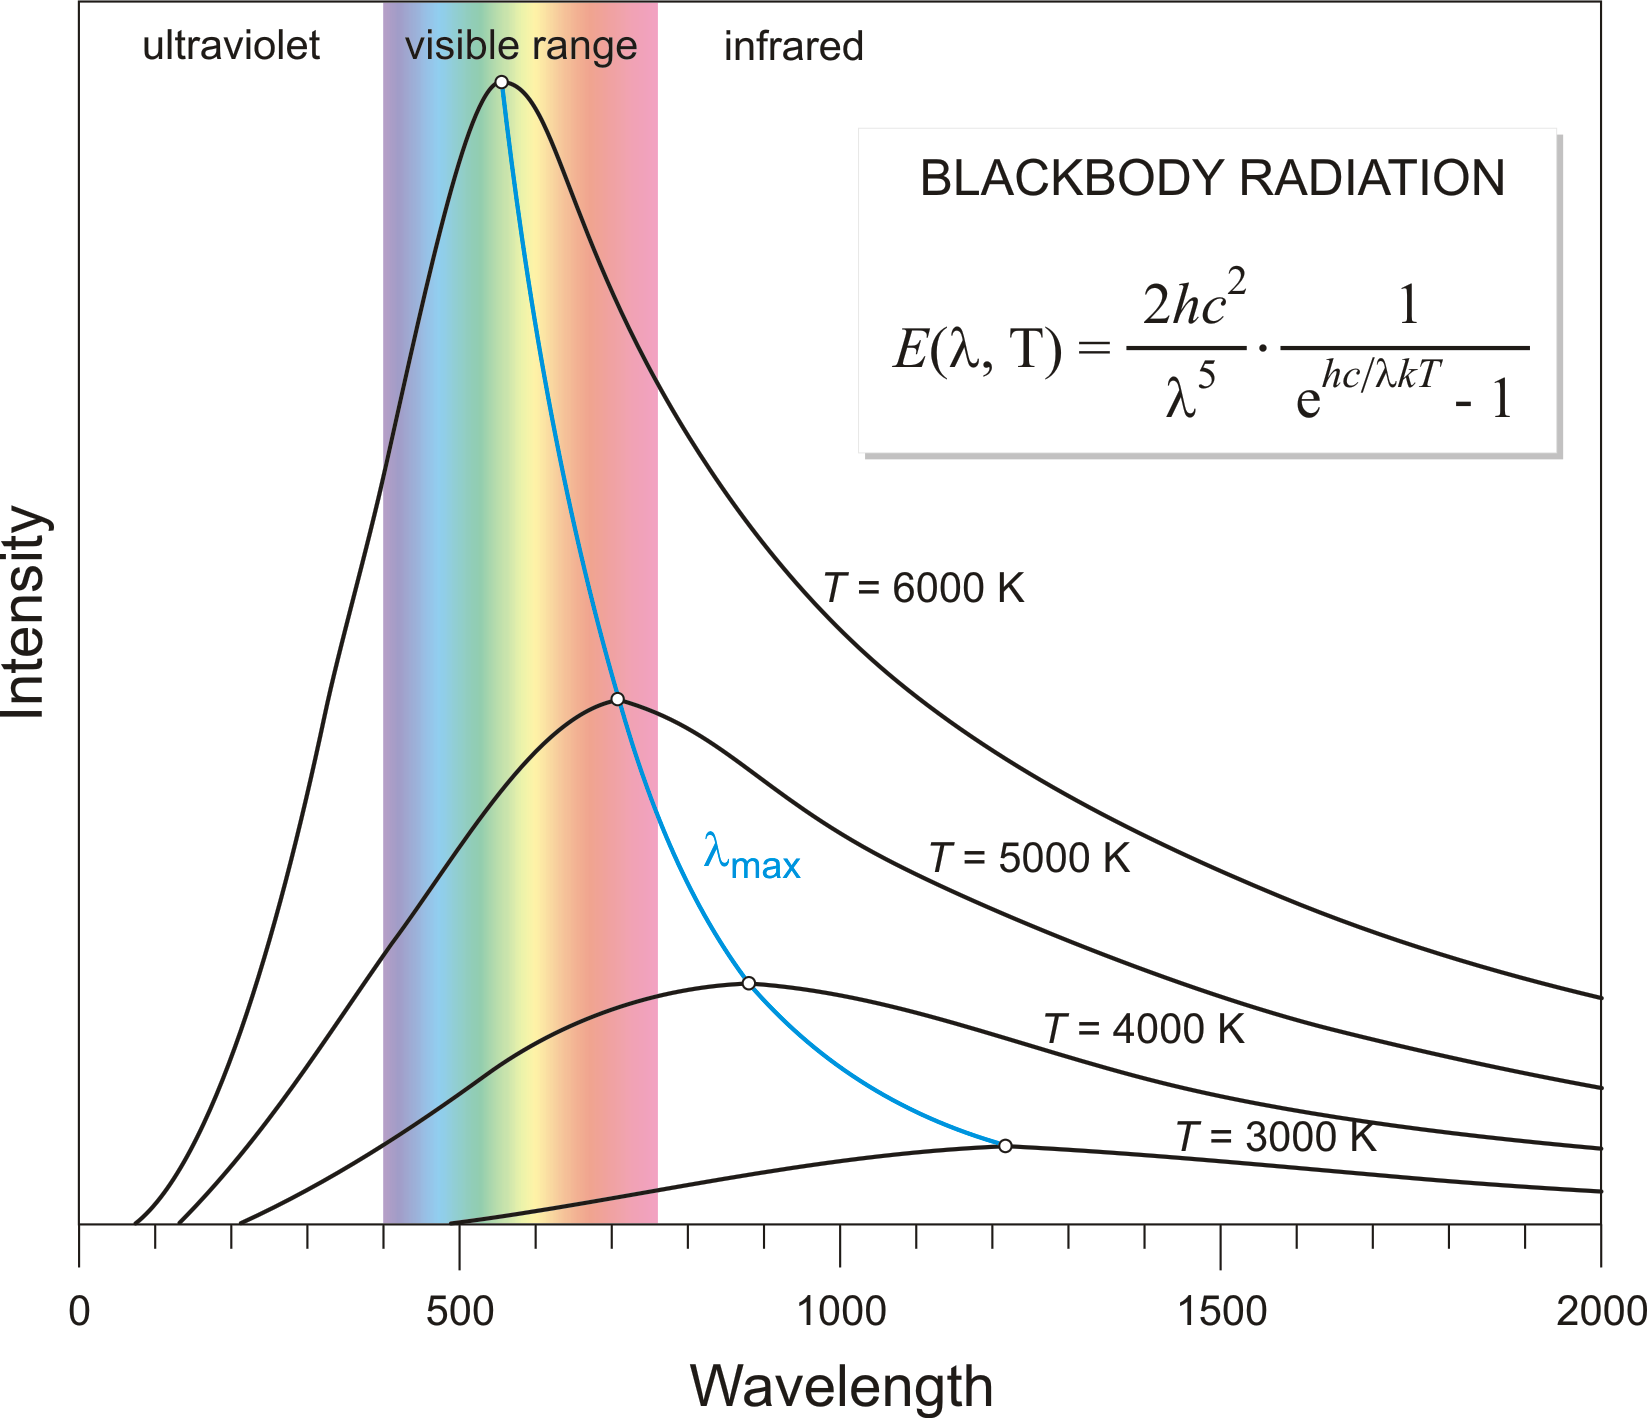
\includegraphics[width=8cm]{blackbody_radiation}
        \caption{A fekete test sugárzás szemléltetése különböző hőmérsékleteken \cite{rad}}
        \label{fig:0blackrad}
    \end{figure}

    A felületre normált sugárzási teljesítményt az $\varepsilon_f$ függvény hullámhossz szerinti integrálja adja meg, melyre érvényes a \textbf{Stefan-Boltzmann-törvény}:
    \begin{equation}
        E_f(T)=\int_{0}^{\infty} \varepsilon_f(\lambda, T)~\mathrm{d}\lambda=\sigma T^4.
    \end{equation}
    Eszerint a kisugárzott teljesítmény arányos a hőmérséklet negyedik hatványával, az arányosssági tényező pedig a \textit{Stefan-Boltzmann-állandó}: $\sigma=5.670\cdot10^{-8}~\frac{W}{m^2K^4}$.
    Egy felületről kisugárzott teljesítmény azonban nem minden irányba azonos, annak szögfüggését a \textit{Lambert-törvény} adja meg:
    \begin{equation}
        \mathrm{d}E_\varphi(T)=\sigma T^4\frac{\cos\varphi}{\pi}\mathrm{d}\Omega,
    \end{equation}
    ahol $\varphi$ a felület normálvektorával bezárt szög, $\mathrm{d}\Omega$ pedig a térszög, amelyet vizsgálunk.

    \subsection{Nem fekete testek sugárzása}
    Két tetszőleges ($1$, $2$) testre a tapasztalat szerint fennáll a következő összefüggés, a hőmérsékleti sugárzás \textit{Kirchhoff-törvénye}:
    \begin{equation}
        \frac{\varepsilon_1(\lambda, T)}{a_1(\lambda, T)}=\frac{\varepsilon_2(\lambda, T)}{a_2(\lambda, T)}=\mathrm{const}.
    \end{equation}
    Mivel ez a fekete testre is érvényes, bármely testre felírható:
    \begin{equation}
        \frac{\varepsilon(\lambda, T)}{a(\lambda, T)}=\varepsilon_f(\lambda, T),
    \end{equation}
    azaz az abszorpció- és emisszióképesség a másik ismeretében meghatározható.

    Szerencsére sok esetben még az egyiket sem kell meghatároznunk minden $\lambda$ értékre, mivel nem túl magas hőmérsékleten sok anyag esetében jó közelítéssel érvényes az $a(\lambda, T)\approx a(T)$ hullámhossz-függés elhanyagolás.
    Az ilyen testeket \textit{szürke testnek} hívjuk (természetesen ez nem a tényleges színre utal).
    Még tovább egyszerűsíthetjük a feladatot alacsony hőmérsékleten, mivel itt legtöbbször az abszorpciós tényező közel konstans, azaz $a(T)\approx a$.

    Ezen közelítések alkalmazásával már könnyen megkapható egy test integrált emisszióképessége:
    \begin{equation}
        E(T)=\int_{0}^{\infty} \varepsilon(\lambda, T)~\mathrm{d}\lambda=\int_{0}^{\infty} a(\lambda, T)\varepsilon_f(\lambda, T)~\mathrm{d}\lambda=a \int_{0}^{\infty} \varepsilon_f(\lambda, T)~\mathrm{d}\lambda,
    \end{equation}
    mely a \textit{Stefan-Boltzmann-törvény} alapján:
    \begin{equation}
        E(T)=a\sigma T^4.
    \end{equation}
    Alacsony hőmérsékletű szürke testekre igaz tehát, hogy integrált emisszióképességük csak egy konstans ($a\in[0, 1]$) szorzóban tér el a fekete testétől.

    \begin{thebibliography}

        \bibitem{leir} \href{https://fizipedia.bme.hu/index.php/H%C5%91m%C3%A9rs%C3%A9kleti_sug%C3%A1rz%C3%A1s_vizsg%C3%A1lata}{Fizipédia, mérési leirat}
        \bibitem{planck} \href{https://en.wikipedia.org/wiki/Planck%27s_law}{A Planck-féle sugárzási törvény}
        \bibitem{rad} \href{https://glossary.periodni.com/glossary.php?en=blackbody+radiation}{A fekete test sugárzása}
    \end{thebibliography}

\end{document}